%% LyX 1.6.4 created this file.  For more info, see http://www.lyx.org/.
%% Do not edit unless you really know what you are doing.
\documentclass[11pt,english]{article}
\usepackage[T1]{fontenc}
\usepackage[latin9]{inputenc}
\usepackage{graphicx}

\makeatletter
%%%%%%%%%%%%%%%%%%%%%%%%%%%%%% User specified LaTeX commands.
%% LyX 1.6.4 created this file.  For more info, see http://www.lyx.org/.
%% Do not edit unless you really know what you are doing.

% ----------------------------------------------------------------

% SIAM packages
%\usepackage[LY1]{fontenc}
%\usepackage[mtbold,LY1]{siammathtime}
\usepackage{epsfig}
\usepackage{graphicx}
\usepackage{makeidx}
\usepackage{multicol}
\usepackage{rotating}
\usepackage{subeqn}
%\usepackage{crop}
\usepackage{url}
\usepackage{longtable}


\newcommand{\basepath}{\path{http://www.cs.utexas.edu/users/flame/}}

% ----------------------------------------------------------------

% Our packages
\usepackage{amssymb}
% \usepackage{graphicx} % already in SIAM
\usepackage{program}
\usepackage{ifthen}
\usepackage{color}
\usepackage{boxedminipage}
% \usepackage[Lenny]{fncychap} % Not necessary with SIAM style
% \usepackage{fancyhdr} % Not necessary with SIAM style
\usepackage{fancyvrb}
% \usepackage{mparhack}
% \usepackage{chappg} % Not necessary with SIAM style
\usepackage[dotinlabels]{titletoc}
\usepackage{colortbl}
\usepackage{array}
\usepackage{soul}
\usepackage{graphics}
\usepackage{moreverb}
\usepackage{fancyhdr}
\usepackage[sf,bf]{titlesec}
\usepackage[Lenny]{fncychap}

\usepackage[dvips,dvipdf,backref,colorlinks,bookmarksopen,bookmarksnumbered,citecolor=blue,urlcolor=blue,backref]{hyperref}

% ----------------------------------------------------------------

% Our macros
\usepackage{ifthen}
\usepackage[dotinlabels]{titletoc}
\usepackage{colortbl}
\usepackage{array}
\usepackage{color}
\usepackage{soul}
\usepackage{amssymb}

% ----------------------------------------------------------------

\newcolumntype{I}{!{\vrule width 1.5pt}}
\newlength\savedwidth
\newcommand\whline{\noalign{\global\savedwidth\arrayrulewidth
                            \global\arrayrulewidth 1.5pt}%
           \hline
           \noalign{\global\arrayrulewidth\savedwidth}}


\newboolean{IsWide}
\setboolean{IsWide}{true}

% In math mode,
% \FlaTwoByTwo{A}{B}
%             {C}{D}
% creates the picture
%   / A || B \
%   | ==  == |
%   \ C || D /

\newcommand{\FlaTwoByTwo}[4]{
\left(
\begin{array}{c I c}
#1 & #2 \\ \whline
#3 & #4
\end{array}
\right)
}

\newcommand{\FlaTwoByTwoNoPar}[4]{
\begin{array}{c I c}
#1 & #2 \\ \whline
#3 & #4
\end{array}
}

\newcommand{\FlaTwoByTwoSingleLineNoPar}[4]{
\begin{array}{c | c}
#1 & #2 \\ \hline
#3 & #4
\end{array}
}

\newcommand{\FlaTwoByTwoSingleLine}[4]{
\left(
\begin{array}{c | c}
#1 & #2 \\ \hline
#3 & #4
\end{array}
\right)
}


\newcommand{\FlaTwoByTwoNoLine}[4]{
\left(
\begin{array}{c  c}
#1 & #2 \\
#3 & #4
\end{array}
\right)
}

% In math mode,
% \FlaTwoByOne{A}
%             {C}
% creates the picture
%   / A  \
%   | == |
%   \ C  /

\newcommand{\FlaTwoByOne}[2]{
\left(
\begin{array}{c}
#1 \\ \whline
#2
\end{array}
\right)
}

\newcommand{\FlaTwoByOneNoPar}[2]{
\begin{array}{c}
#1 \\ \whline
#2
\end{array}
}

% In math mode,
% \FlaTwoByOneSingleLine{A}
%                       {C}
% creates the picture
%   / A  \
%   | -- |
%   \ C  /

\newcommand{\FlaTwoByOneSingleLine}[2]{
\left(
\begin{array}{c}
#1 \\ \hline
#2
\end{array}
\right)
}


\newcommand{\FlaTwoByOneNoLine}[2]{
\left(
\begin{array}{c}
#1 \\
#2
\end{array}
\right)
}

% In math mode,
% \FlaOneByTwo{A}{B}
% creates the picture
%   ( A || B )

\newcommand{\FlaOneByTwo}[2]{
\left(
\begin{array}{c I c}
#1 & #2
\end{array}
\right)
}

\newcommand{\FlaOneByTwoNoPar}[2]{
\begin{array}{c I c}
#1 & #2
\end{array}
}

\newcommand{\FlaOneByTwoSingleLine}[2]{
\left(
\begin{array}{c | c}
#1 & #2
\end{array}
\right)
}

\newcommand{\FlaOneByTwoNoLine}[2]{
\left(
\begin{array}{c c}
#1 & #2
\end{array}
\right)
}

% In math mode,
% \FlaThreeByThreeTL{A}{B}{C}
%                   {D}{E}{F}
%                   {G}{H}{I}
% creates the picture
%   / A | B || C \
%   | -- ---  -- |
%   | D | E || F |
%   | ==  ==  == |
%   \ G | H || I /
% Notice: the TL means that the
% center block (E) is part of the
% TL quadrant, where quadrants are
% partitioned by the double lines.

\newcommand{\FlaThreeByThreeTL}[9]{
\left(
\begin{array}{c | c I c}
#1 & #2 & #3 \\ \hline
#4 & #5 & #6 \\ \whline
#7 & #8 & #9
\end{array}
\right)
}

% In math mode,
% \FlaThreeByThreeBR{A}{B}{C}
%                   {D}{E}{F}
%                   {G}{H}{I}
% creates the picture
%   / A || B | C \
%   | ==  ==  == |
%   | D || E | F |
%   | -- ---  -- |
%   \ G || H | I /
% Notice: the BR means that the
% center block (E) is part of the
% BR quadrant, where quadrants are
% partitioned by the double lines.

\newcommand{\FlaThreeByThreeBR}[9]{
\left(
\begin{array}{c I c | c}
#1 & #2 & #3 \\ \whline
#4 & #5 & #6 \\ \hline
#7 & #8 & #9
\end{array}
\right)
}

\newcommand{\FlaThreeByThreeSingleLine}[9]{
\left(
\begin{array}{c | c | c}
#1 & #2 & #3 \\ \hline
#4 & #5 & #6 \\ \hline
#7 & #8 & #9
\end{array}
\right)
}

\newcommand{\FlaThreeByThreeNoLine}[9]{
\left(
\begin{array}{c c c}
#1 & #2 & #3 \\
#4 & #5 & #6 \\
#7 & #8 & #9
\end{array}
\right)
}

% In math mode,
% \FlaThreeByThreeTR{A}{B}{C}
%                   {D}{E}{F}
%                   {G}{H}{I}
% creates the picture
%   / A || B | C \
%   | -- ---  -- |
%   | D || E | F |
%   | ==  ==  == |
%   \ G || H | I /
% Notice: the TR means that the
% center block (E) is part of the
% TR quadrant, where quadrants are
% partitioned by the double lines.

\newcommand{\FlaThreeByThreeTR}[9]{
\left(
\begin{array}{c I c | c}
#1 & #2 & #3 \\ \hline
#4 & #5 & #6 \\ \whline
#7 & #8 & #9
\end{array}
\right)
}


% In math mode,
% \FlaThreeByThreeBL{A}{B}{C}
%                   {D}{E}{F}
%                   {G}{H}{I}
% creates the picture
%   / A | B || C \
%   | ==  ==  == |
%   | D | E || F |
%   | -- ---  -- |
%   \ G | H || I /
% Notice: the BL means that the
% center block (E) is part of the
% BL quadrant, where quadrants are
% partitioned by the double lines.

\newcommand{\FlaThreeByThreeBL}[9]{
\left(
\begin{array}{c | c I c}
#1 & #2 & #3 \\ \whline
#4 & #5 & #6 \\ \hline
#7 & #8 & #9
\end{array}
\right)
}

% In math mode,
% \FlaOneByThreeR{A}{B}{C}
% creates the picture
%   ( A || B | C )
% Notice: the R means that the
% center block (B) is part of the
% R(ight) submatrix, where
% submatrices are % partitioned
% by the double lines.

\newcommand{\FlaOneByThreeR}[3]{
\left(
\begin{array}{c I c | c}
#1 & #2 & #3
\end{array}
\right)
}

% In math mode,
% \FlaOneByThreeL{A}{B}{C}
% creates the picture
%   ( A | B || C )
% Notice: the R means that the
% center block (B) is part of the
% R(ight) submatrix, where
% submatrices are % partitioned
% by the double lines.

\newcommand{\FlaOneByThreeL}[3]{
\left(
\begin{array}{c | c I c}
#1 & #2 & #3
\end{array}
\right)
}

% In math mode,
% \FlaThreeByOneT{A}
%                {D}
%                {G}
% creates the picture
%   / A  \
%   | == |
%   | B  |
%   | -- |
%   \ C  /
% Notice: the T means that the
% center block (C) is part of the
% T(op) submatrix where submatrices
% are % partitioned by the double
% lines.

\newcommand{\FlaThreeByOneT}[3]{
\left(
\begin{array}{c}
#1 \\ \hline
#2 \\ \whline
#3
\end{array}
\right)
}

\newcommand{\FlaThreeByOneTNoPar}[3]{
\begin{array}{c}
#1 \\ \hline
#2 \\ \whline
#3
\end{array}
}

% In math mode,
% \FlaThreeByOneB{A}
%                {D}
%                {G}
% creates the picture
%   / A  \
%   | -- |
%   | B  |
%   | == |
%   \ C  /
% Notice: the B means that the
% center block (C) is part of the
% T(op) submatrix where submatrices
% are % partitioned by the double
% lines.

\newcommand{\FlaThreeByOneB}[3]{
\left(
\begin{array}{c}
#1 \\ \whline
#2 \\ \hline
#3
\end{array}
\right)
}

\newcommand{\FlaThreeByOneBNoPar}[3]{
\begin{array}{c}
#1 \\ \whline
#2 \\ \hline
#3
\end{array}
}

\newcommand{\FlaThreeByOneSingleLine}[3]{
\left(
\begin{array}{c}
#1 \\ \hline
#2 \\ \hline
#3
\end{array}
\right)
}

\newcommand{\FlaThreeByOneNoLine}[3]{
\left(
\begin{array}{c}
#1 \\
#2 \\
#3
\end{array}
\right)
}

% Various key words

% The following is a typical use of
% \FlaPartition:
%
% \FlaPartition {
%    $ A \rightarrow \FlaTwoByTwo{ A_{TL} }{ A_{TR} }
%                                { A_{BL} }{ A_{BR} } $
% }
% {
%    where $ A_{TL} $ is $ 0 \times 0 $
% }
%
% Creates something like
% Partition A -> / A_TL || A_TR \
%                | =====  ===== |
%                \ A_BL || A_BR /
% where A_TL is 0 x 0
%

\newcommand{\FlaPartition}[2]{
\ifthenelse{\boolean{IsWide}}{{\bf partition } \hspace{-1em} #1 \hspace{-1em} #2}
{{\bf partition } \+ \\ #1 \+ \\ #2 \- \-}
}

% The following is a typical use of
% \FlaRepartition:
%
% \FlaRepartition{
% $
% \FlaTwoByTwo{ A_{TL} }{ A_{TR} }
%             { A_{BL} }{ A_{BR} } \rightarrow
% \FlaThreeByThreeBR{ A_{00} }{ A_{01} }{ A_{02} }
%                   { A_{10} }{ A_{11} }{ A_{12} }
%                   { A_{20} }{ A_{21} }{ A_{22} }
% $
% }
% {
%    \FlaWhere{$ A_{11} $ is $ b \times b $}
%  }
%
% Creates something like
% Repartition
%   / A_TL || A_TR \    / A_00 || A_01 | A_02 \
%   | =====  ===== | -> | =====  ====== ===== |
%   \ A_BL || A_BR /    | A_10 || A_11 | A_12 |
%                       | -----  ------ ----- |
%                       \ A_20 || A_21 | A_22 /
% where A_11 is b x b
%

\newcommand{\FlaRepartition}[2]{
\ifthenelse{\boolean{IsWide}}{{\bf repartition } \hspace{-1em} #1 \hspace{-1em} #2}
{{\bf repartition } \+ \\ #1 \+ \\ #2 \- \-}
}

% The following is a typical use of
% \FlaContinue:
%
% \FlaContinue{
% $
%    \FlaTwoByTwo{ A_{TL} }{ A_{TR} }
%                { A_{BL} }{ A_{BR} } \leftarrow
%    \FlaThreeByThreeTL{ A_{00} }{ A_{01} }{ A_{02} }
%                      { A_{10} }{ A_{11} }{ A_{12} }
%                      { A_{20} }{ A_{21} }{ A_{22} }
% $
% }
%
% Creates something like
% Continue with
%   / A_TL || A_TR \    / A_00 | A_01 || A_02 \
%   | =====  ===== | <- | ----- ------  ----- |
%   \ A_BL || A_BR /    | A_10 | A_11 || A_12 |
%                       | ===== ======  ===== |
%                       \ A_20 | A_21 || A_22 /

\newcommand{\FlaStartCompute}{%
\setlength{\unitlength}{3in}%
\begin{picture}(2,0.01)
\put(0,0){\line(1,0){2}}
\put(0,0.01){\line(1,0){2}}
\end{picture}%
}

\newcommand{\FlaEndCompute}{%
\noindent%
\setlength{\unitlength}{3in}%
\begin{picture}(2,0.01)
\put(0,0){\line(1,0){2}}
\put(0,0.01){\line(1,0){2}}
\end{picture}%
}

\newcommand{\FlaStartComputeShort}{
\setlength{\unitlength}{1.30in}
\begin{picture}(3,0.01)
\put(0,0){\line(1,0){3}}
\put(0,0.01){\line(1,0){3}}
\end{picture}
}

\newcommand{\FlaStartComputeShorter}{
{\color{red}
\setlength{\unitlength}{0.5in}
\begin{picture}(3,0.01)
\put(0,0){\line(1,0){3}}
\put(0,0.01){\line(1,0){3}}
\end{picture}
}
}

\newcommand{\FlaEndComputeShort}{
\setlength{\unitlength}{1.30in}
\begin{picture}(3,0.01)
\put(0,0){\line(1,0){3}}
\put(0,0.01){\line(1,0){3}}
\end{picture}
}

\newcommand{\FlaEndComputeShorter}{
{\color{red}
\setlength{\unitlength}{0.5in}
\begin{picture}(3,0.01)
\put(0,0){\line(1,0){3}}
\put(0,0.01){\line(1,0){3}}
\end{picture}
}
}

\newcommand{\FlaUpLo}[2]{
{#1} \backslash {#2}
}

\newcommand{\FlaInverse}[1]{
{ #1 }^{-1}
}

\newcommand{\Square}{ \mbox{Square} }
\newcommand{\Symm}{ \mbox{Symm} }
\newcommand{\SameSize}{ \mbox{SameSize} }
\newcommand{\RowDim}{\mbox{RowDim}}
\newcommand{\ColDim}{\mbox{ColDim}}
\newcommand{\LowTr}{\mbox{LowTr}}
\newcommand{\UpTr}{\mbox{UpTr}}
\newcommand{\UpperTr}{\mbox{UpTr}}
\newcommand{\UppTr}{\mbox{UpTr}}
\newcommand{\operation}{ [ D, E, F, \ldots ] \becomes {\rm op}( A, B, C, D, \ldots ) }
\newcommand{\routinename}{ [ D, E, F, \ldots ] \becomes {\rm op}( A, B, C, D, \ldots ) }
\newcommand{\routinecost}{ X }
\newcommand{\precondition}{ Q }
\newcommand{\postcondition}{ R }
\newcommand{\invariant}{ P }
\newcommand{\costinv}{ \  }
\newcommand{\costbefore}{ \  }
\newcommand{\costafter}{ \  }
\newcommand{\updatecost}{ \  }
\newcommand{\guard}{ R }
\newcommand{\partitionings}{
\begin{minipage}{3in}
$ S_I $
\end{minipage}
}
\newcommand{\partitionsizes}{ \hspace{ 3.25in} }

\newcommand{\blocksize}{1}

\newcommand{\repartitionings}{
\begin{minipage}[t]{3in}
\ \\
\ \\
\ \\
\end{minipage}
}

\newcommand{\repartitionsizes}{ \hspace{ 3.25in} }
\newcommand{\moveboundaries}{
\begin{minipage}[t]{3in}
\ \\
\ \\
\ \\
\end{minipage}
}
\newcommand{\beforeupdate}{
$ \QBefore $
}
\newcommand{\afterupdate}{
$ \QAfter $
}
\newcommand{\update}{%
\begin{minipage}[t]{4in}
$ S_U $
\end{minipage}
}

\newcommand{\resetsteps}{
\renewcommand{\blocksize}{1}
\renewcommand{\operation}{ [ D, E, F, \ldots ] \becomes {\rm op}( A, B, C, D, \ldots ) }
\renewcommand{\routinename}{ [ D, E, F, \ldots ] \becomes {\rm op}( A, B, C, D, \ldots ) }
\renewcommand{\routinecost}{ 0 }
\renewcommand{\precondition}{ \PPre }
\renewcommand{\postcondition}{ \PPost }
\renewcommand{\invariant}{ \PInv }
\renewcommand{\costinv}{ \  }
\renewcommand{\guard}{ G }
\renewcommand{\partitionings}{ %
\begin{minipage}[t]{3in}
\ \\
\end{minipage}
}
\renewcommand{\partitionsizes}{ \hspace{ 3.25in} }
\renewcommand{\repartitionings}{%
\begin{minipage}[t]{3in}
\ \\
\end{minipage}
}
\renewcommand{\repartitionsizes}{ \hspace{ 3.25in} }
\renewcommand{\moveboundaries}{%
\begin{minipage}[t]{3in}
\ \\
\end{minipage}
}
\renewcommand{\beforeupdate}{
\QBefore
}
\renewcommand{\afterupdate}{
\QAfter
}
\renewcommand{\update}{
$ S_U $
}
}

\newenvironment{FlaBox}{
\footnotesize
\begin{framebox}
}
{
\end{framebox}
}

\newcommand{\WSoperation}{
$ \operation $
}

\newcommand{\WSprecondition}{
$ \left\{ \precondition \right\} $
}

\newcommand{\WSpostcondition}{
$ \left\{ \postcondition \right\} $
}

\newcommand{\WSinvariant}{
$ \left\{ \invariant \right\} $
}

\newcommand{\WScostinv}{
$ \Csf = \costinv $ flops
}

\newcommand{\WScostzero}{
$ \Csf = 0 $ flops
}

\newcommand{\WScostbu}{
$ \Csf = \costbefore $ flops
}

\newcommand{\WScostau}{
$ \Csf = \costafter $ flops
}

\newcommand{\WSupdatecost}{
{\bf Cost:} $ \updatecost $ flops
}

\newcommand{\WStopofloop}{
$ \left\{ \left( \invariant \right) \wedge \left( \guard \right) \right\} $
}

\newcommand{\WStopofloopnarrow}{
$ \begin{array}{r}
  \left\{ \left( \invariant \right) \right. \\
  \left. \wedge \left( \guard \right) \right\}
\end{array} $
}

\newcommand{\WSafterloop}{
$ \left\{ \left( \invariant \right) \wedge \neg \left( \guard \right) \right\} $
}

\newcommand{\WSguard}{
$ \guard $
}

\newcommand{\WSpartition}{
\begin{minipage}[t]{3in}
\begin{tabbing}
ind \= ind \= \kill
{\bf \color{blue} Partition}
\partitionings \+ \\
{\bf \color{blue} where } \hspace*{-2ex} \partitionsizes
\end{tabbing}
\end{minipage}
}

\newcommand{\WSpartitionNarrow}{
\begin{minipage}[t]{2.0in}
\begin{tabbing}
id \= id \= \kill
{\bf \color{blue} Partition}
\partitionings \+ \\
{\bf \color{blue} where }
\begin{minipage}[t]{1.5in}
\partitionsizes
\end{minipage}
\end{tabbing}
\end{minipage}
}

\newcommand{\WSrepartition}{
\begin{minipage}[t]{3in}
\ifthenelse{ \equal{\blocksize}{1} }{}
{%
\ifthenelse{ \equal{\blocksize}{blank} }{~}
{{\bf Determine block size $ \blocksize $}} \\
}
{\bf \color{blue} Repartition}
\begin{tabbing}
in \= in \= \+ \kill
\repartitionings \+ \\
{\bf \color{blue} where } \hspace*{-2ex} \repartitionsizes
\end{tabbing}
\end{minipage}
}

\newcommand{\WSrepartitionNarrow}{
\begin{minipage}[t]{2.05in}
\ifthenelse{ \equal{\blocksize}{1} }{}
{%
\ifthenelse{ \equal{\blocksize}{blank} }{~}
{{\bf \color{blue} Determine block size $ \blocksize $}} \\
}
{\bf \color{blue} Repartition}
\begin{tabbing}
i \= i \= \+ \kill
\repartitionings \+ \\
{\bf \color{blue} where }
\begin{minipage}[t]{1.5in}
\repartitionsizes
\end{minipage}
\end{tabbing}
\end{minipage}
}

\newcommand{\WSmoveboundary}{
\begin{minipage}[t]{4in}
{\bf \color{blue} Continue with}
\begin{tabbing}
ind \= \+ \kill
\moveboundaries
\end{tabbing}
\end{minipage}
}

\newcommand{\WSmoveboundaryNarrow}{
\begin{minipage}[t]{2.05in}
{\bf \color{blue} Continue with}
\begin{tabbing}
i \= \+ \kill
\moveboundaries
\end{tabbing}
\end{minipage}
}

\newcommand{\WSbeforeupdate}{
$ \left\{ \beforeupdate \right\} $
}

\newcommand{\WSafterupdate}{
$ \left\{ \afterupdate \right\} $
}

\newcommand{\WSupdate}{
\update
}

\newcommand{\worksheet}{
\begin{center}
\begin{tabular}{| c I l |} \hline
\footnotesize {\bf Step} &
{\bf \color{blue} Annotated Algorithm:} $\operation$
\\ \whline
\rowcolor[gray]{0.93}
1a &
\WSprecondition \\ \hline
4 &
\WSpartition \\ \hline
\rowcolor[gray]{0.93}
2 &
\WSinvariant \\ \hline
3 &
{\bf \color{blue} while} \WSguard { \bf \color{blue} do} \\ \hline
\rowcolor[gray]{0.93}
2,3 &
\ \hspace{0.15in} \WStopofloop \\ \hline
5a &
\ \hspace{0.15in}
\WSrepartition
\\ \hline
\rowcolor[gray]{0.93}
6 &
\ \hspace{0.15in} \WSbeforeupdate \\ \hline
8 & \ \hspace{0.15in} \WSupdate \\ \hline
5b &
\ \hspace{0.15in}
\WSmoveboundary
\\ \hline
\rowcolor[gray]{0.93}
7 &
\ \hspace{0.15in} \WSafterupdate \\ \hline
\rowcolor[gray]{0.93}
2 &
\ \hspace{0.15in} \WSinvariant \\ \hline
& {\bf \color{blue} endwhile} \\ \hline
\rowcolor[gray]{0.93}
2,3 &
\WSafterloop \\ \hline
\rowcolor[gray]{0.93}
1b &
\WSpostcondition \\ \hline
\end{tabular}
\end{center}
}

\newcommand{\worksheetnarrow}{
\begin{center}
\begin{tabular}{| c I l |} \hline
\footnotesize {\bf Step} &
{\bf \color{blue} Annotated Algorithm:} $\routinename$
\\ \whline
\rowcolor[gray]{0.93}
1a &
\WSprecondition \\ \hline
4 &
\WSpartition \\ \hline
\rowcolor[gray]{0.93}
2 &
\WSinvariant \\ \hline
3 &
{\bf \color{blue} while} \WSguard { \bf \color{blue} do} \\ \hline
\rowcolor[gray]{0.93}
2,3 &
\ \hspace{0.15in} \WStopofloopnarrow \\ \hline
5a &
\ \hspace{0.15in}
\WSrepartition
\\ \hline
\rowcolor[gray]{0.93}
6 &
\ \hspace{0.15in} \WSbeforeupdate \\ \hline
8 & \ \hspace{0.15in} \WSupdate \\ \hline
5b &
\ \hspace{0.15in}
\WSmoveboundary
\\ \hline
\rowcolor[gray]{0.93}
7 &
\ \hspace{0.15in} \WSafterupdate \\ \hline
\rowcolor[gray]{0.93}
2 &
\ \hspace{0.15in} \WSinvariant \\ \hline
& {\bf \color{blue} endwhile} \\ \hline
\rowcolor[gray]{0.93}
2,3 &
\WSafterloop \\ \hline
\rowcolor[gray]{0.93}
1b &
\WSpostcondition \\ \hline
\end{tabular}
\end{center}
}

\newcommand{\worksheetwithcost}{
\begin{center}
\begin{tabular}{| c I l  r | } \hline
\footnotesize {\bf Step} &
\multicolumn{2}{l|}
{{\bf Cost Analysis:} $\routinename$}
\\ \whline
\rowcolor[gray]{0.93}
1a &
% \WSprecondition
& \WScostzero \\ \hline
4 & \multicolumn{2}{l|}{
\WSpartition} \\ \hline
\rowcolor[gray]{0.93}
2 &
% \WSinvariant
& \WScostinv \\ \hline
3 & \multicolumn{2}{l|}{
{\bf \color{blue} while} \WSguard { \bf \color{blue} do} }\\ \hline
\rowcolor[gray]{0.93}
2,3 &
% \ \hspace{0.15in} \WStopofloop
& \WScostinv \\ \hline
5a & \multicolumn{2}{l|}{
\ \hspace{0.15in}
\WSrepartition}
\\ \hline
\rowcolor[gray]{0.93}
6 &
% \ \hspace{0.15in} \WSbeforeupdate
&
\WScostbu
\\ \hline
8 &
\hspace{0.15in} \WSupdate
&
\WSupdatecost \\ \hline
5b &\multicolumn{2}{l|}{
\ \hspace{0.15in}
\WSmoveboundary}
\\ \hline
\rowcolor[gray]{0.93}
7 &
% \ \hspace{0.15in} \WSafterupdate
&
\WScostau
\\ \hline
\rowcolor[gray]{0.93}
2 &
% \ \hspace{0.15in} \WSinvariant
&
\WScostinv \\ \hline
& \multicolumn{2}{l|}{{\bf \color{blue} endwhile}} \\ \hline
\rowcolor[gray]{0.93}
2,3 &
% \WSafterloop
&
\WScostinv
\\ \hline
\rowcolor[gray]{0.93}
1b &
% \WSpostcondition
\multicolumn{2}{r|}
{{\bf Total Cost:} $ \routinecost $ flops}
\\ \hline
\end{tabular}
\end{center}
}

\newcommand{\worksheetnosteps}{
\begin{center}
\begin{tabular}{| l |} \hline
{ \color{blue} Annotated Algorithm: } \WSoperation \\ \whline
\rowcolor[gray]{0.93}
\WSprecondition \\ \hline
\WSpartition \\ \hline
\rowcolor[gray]{0.93}
\WSinvariant \\ \hline
{\bf \color{blue} while} \WSguard { \bf \color{blue} do} \\ \hline
\rowcolor[gray]{0.93}
\ \hspace{0.15in} \WStopofloop \\ \hline
\ \hspace{0.15in}
\WSrepartition
\\ \hline
\rowcolor[gray]{0.93}
\ \hspace{0.15in} \WSbeforeupdate \\ \hline
\hspace{0.15in} \WSupdate \\ \hline
\ \hspace{0.15in}
\WSmoveboundary
\\ \hline
\rowcolor[gray]{0.93}
\ \hspace{0.15in} \WSafterupdate \\ \hline
\rowcolor[gray]{0.93}
\ \hspace{0.15in} \WSinvariant \\ \hline
{\bf \color{blue} endwhile} \\ \hline
\rowcolor[gray]{0.93}
\WSafterloop \\ \hline
\rowcolor[gray]{0.93}
\WSpostcondition \\ \hline
\end{tabular}
\end{center}
}

\newcommand{\worksheetupdate}{
\begin{center}
\begin{tabular}{| c I l |} \hline
\footnotesize Step & { \color{blue} Annotated Algorithm: } \WSoperation \\ \whline
3 &
{\bf \color{blue} while} \WSguard { \bf \color{blue} do} \\ \hline
2,3 &
\ \hspace{0.15in} \WStopofloop \\ \hline
5a &
\ \hspace{0.15in}
\WSrepartition
\\ \hline
6 &
\ \hspace{0.15in} \WSbeforeupdate \\ \hline
8 & \hspace{0.15in} \WSupdate \\ \hline
5b &
\ \hspace{0.15in}
\WSmoveboundary
\\ \hline
7 &
\ \hspace{0.15in} \WSafterupdate \\ \hline
2 &
\ \hspace{0.15in} \WSinvariant \\ \hline
& {\bf \color{blue} endwhile} \\ \hline
\end{tabular}
\end{center}
}

\newcommand{\FlaAlgorithm}{
\begin{center}
\begin{tabular}{|l |} \hline
{\bf \color{blue} Algorithm:} $\routinename$
\\ \whline
{\WSpartition} \\[0.3in]
{\bf \color{blue} while} \WSguard { \bf \color{blue} do} \\
\ \hspace{0.15in} \WSrepartition \\
\color{red} {\hspace{0.0in} \FlaStartCompute} \\
{\hspace{0.0in} \WSupdate} \\
\color{red} {\hspace{0.0in} \FlaEndCompute} \\
{\ \hspace{0.15in} \WSmoveboundary} \\
{{\bf \color{blue} endwhile}} \\ \hline
\end{tabular}
\end{center}
}


\newcommand{\FlaAlgorithmNarrow}{
\begin{center}
\begin{tabular}{|l |} \hline
{\bf \color{blue} Algorithm:} $\routinename$
\\ \whline
{\WSpartitionNarrow} \\
{\bf \color{blue} while} \WSguard { \bf \color{blue} do} \\
\ \hspace{0.0in} \WSrepartitionNarrow \\
{\hspace{0.0in} \FlaStartComputeShorter} \\
{\hspace{0.0in} \WSupdate} \\
{\hspace{0.0in} \FlaEndComputeShorter} \\
{\ \hspace{0.0in} \WSmoveboundaryNarrow} \\
{{\bf \color{blue} endwhile}} \\ \hline
\end{tabular}
\end{center}
}


\newcommand{ \PPre }{ P_{\it pre} }
\newcommand{ \PPost }{ P_{\it post} }
\newcommand{ \PInv }{ P_{\it inv} }
\newcommand{ \PInvone }{ P_{\it inv-1} }
\newcommand{ \PInvtwo }{ P_{\it inv-2} }
\newcommand{ \becomes }{:=}
\newcommand{ \QBefore }{ P_{\it before} }
\newcommand{ \QAfter }{ P_{\it after} }
\newcommand{ \Qbefore }{ P_{\it before} }
\newcommand{ \Qafter }{ P_{\it after} }
\newcommand{ \PCons }{ P_{\it cons} }
\newcommand{ \PCost }{ P_{\it cost} }
\newcommand{ \PStr }{ P_{\it struct} }
\newcommand{ \Csf }{ C_{\it sf} }

% THEOREMS -------------------------------------------------------


\newcommand{\FlaComputeSection}[1]{
\color{red}
\setlength{\unitlength}{#1}
\begin{picture}(1,0.01)
\put(0,0){\line(1,0){1}}
\put(0,0.01){\line(1,0){1}}
\end{picture}
}

\newcommand{\routinenameL}{}
\newcommand{\routinenameR}{}

\newcommand{\partitioningsL}{}
\newcommand{\partitioningsR}{}

\newcommand{\partitionsizesL}{}
\newcommand{\partitionsizesR}{}

\newcommand{\repartitioningsL}{}
\newcommand{\repartitioningsR}{}

\newcommand{\repartitionsizesL}{}
\newcommand{\repartitionsizesR}{}

\newcommand{\blocksizeL}{}
\newcommand{\blocksizeR}{}

\newcommand{\moveboundariesL}{}
\newcommand{\moveboundariesR}{}

\newcommand{\updateL}{}
\newcommand{\updateR}{}

\newcommand{\WSpartitionNarrowL}{
\begin{minipage}[t]{2.0in}
\begin{tabbing}
id \= id \= \kill
{\bf \color{blue} Partition} 
\partitioningsL \+ \\
{\bf \color{blue} where } 
\begin{minipage}[t]{2in}
\partitionsizesL 
\end{minipage}
\end{tabbing}
\end{minipage}
}

\newcommand{\WSpartitionNarrowR}{
\begin{minipage}[t]{2.0in}
\begin{tabbing}
id \= id \= \kill
{\bf Partition} 
\partitioningsR \+ \\
{\bf where} 
\begin{minipage}[t]{2in}
\partitionsizesR 
\end{minipage}
\end{tabbing}
\end{minipage}
}


\newcommand{\WSrepartitionNarrowL}{
\begin{minipage}[t]{2.05in}
{\bf \color{blue} Repartition}
\begin{tabbing}
i \= i \= \+ \kill
\repartitioningsL \+ \\
{\bf \color{blue} where}
\begin{minipage}[t]{2in}
\repartitionsizesL
\end{minipage}
\end{tabbing}
\end{minipage}
}


\newcommand{\WSrepartitionNarrowR}{
\begin{minipage}[t]{2.05in}
{\bf \color{blue} Repartition}
\begin{tabbing}
i \= i \= \+ \kill
\repartitioningsR \+ \\
{\bf \color{blue} where}
\begin{minipage}[t]{2in}
\repartitionsizesR
\end{minipage}
\end{tabbing}
\end{minipage}
}


\newcommand{\WSblocksizeL}{
\ifthenelse{ \equal{\blocksizeL}{1}}{}
{%
\ifthenelse{ \equal{\blocksizeL}{blank} }{}
}
{{\bf \color{blue} Determine block size $ \blocksizeL $}} 
}

\newcommand{\WSblocksizeR}{
\ifthenelse{ \equal{\blocksizeR}{1} }{}
{%
\ifthenelse{ \equal{\blocksizeR}{blank} }{}
}
{{\bf \color{blue} Determine block size $ \blocksizeR $}} 
}


\newcommand{\WSmoveboundaryNarrowL}{
\begin{minipage}[t]{2.05in}
{\bf \color{blue} Continue with}
\begin{tabbing}
i \= \+ \kill
\moveboundariesL 
\end{tabbing}
\end{minipage}
}



\newcommand{\WSmoveboundaryNarrowR}{
\begin{minipage}[t]{2.05in}
{\bf Continue with}
\begin{tabbing}
i \= \+ \kill
\moveboundariesR 
\end{tabbing}
\end{minipage}
}


\newcommand{\WSupdateL}{
\updateL
}

\newcommand{\WSupdateR}{
\updateR
}


\newcommand{\FlaAlgorithmTwo}{
\begin{center}
\begin{tabular}{| p{3.0in} | @{}c@{} | p{3.0in} |} 
\cline{1-1} \cline{3-3}
% {\bf \color{blue} Algorithm:} 
$\routinenameL$
&
~
&
% {\bf \color{blue} Algorithm:} 
$\routinenameR$
\\ \cline{1-1} \cline{3-3}
\begin{tabular}{@{}l}
\WSpartitionNarrowL
\end{tabular}
&
&
\begin{tabular}{@{}l}
\WSpartitionNarrowR
\end{tabular}
\\
{\bf \color{blue} while} \WSguard { \bf \color{blue} do} 
&
&
{\bf \color{blue} while} \WSguard { \bf \color{blue} do} \\
\ifthenelse{ \equal{\blocksizeL}{blank} }{
\ifthenelse{ \equal{\blocksizeR}{blank} }{}
{
\ \hspace{0.0in} \WSblocksizeL
&
&
\ \hspace{0.0in} \WSblocksizeR
\\}
}
\ \hspace{0.0in} \WSrepartitionNarrowL 
&
&
\ \hspace{0.0in} \WSrepartitionNarrowR 
\\
{\hspace{0.0in} \FlaComputeSection{2.75in} }
&
&
{\hspace{0.0in} \FlaComputeSection{2.75in} }
\\
{\hspace{0.0in} \WSupdateL} 
&
&
{\hspace{0.0in} \WSupdateR} 
\\
{\hspace{0.0in} \FlaComputeSection{2.75in} }
&
&
{\hspace{0.0in} \FlaComputeSection{2.75in} }
\\
{\ \hspace{0.0in} \WSmoveboundaryNarrowL} 
&
&
{\ \hspace{0.0in} \WSmoveboundaryNarrowR} 
\\
{{\bf \color{blue} endwhile}} 
&
&
{{\bf \color{blue} endwhile}} 
\\ \cline{1-1} \cline{3-3}
\end{tabular}
\end{center}
}

% THEOREMS -------------------------------------------------------

\setlength{\topsep}{0pt}
%\newtheorem{theorem}{Theorem}[chapter] % already in SIAM macros
%\newtheorem{algorithm}[theorem]{Algorithm} % already in SIAM macros
%\newtheorem{lemma}[theorem]{Lemma} % already in SIAM macros
%\newtheorem{corollary}[theorem]{Corollary} % already in SIAM macros
%%\newtheorem{example}{Example} % already in SIAM macros
%\newtheorem{example}[theorem]{Example} % already in SIAM macros
%\newtheorem{definition}[theorem]{Definition} % already in SIAM macros
%%\newtheorem{definition}{Definition} % already in SIAM macros
%\newtheorem{remark}[theorem]{Remark}
%\newtheorem{exercise}[theorem]{Exercise}
%% \renewenvironment{proof}{\noindent
%% {\bf Proof:}}
%% {\hfill {\bf endofproof}}

\newenvironment{boxedexample}{
\noindent
\newline
\begin{boxedminipage}[t]{\textwidth}
\addtocounter{ourexample}{1}%
{\bf Example \thechapter.\theourexample.}
\em
}
{
\end{boxedminipage}
}

\newenvironment{boxedexercise}{
\noindent
\newline
\begin{boxedminipage}[t]{\textwidth}
\begin{exercise}
}
{
\end{exercise}
\end{boxedminipage}
}

\newenvironment{boxit}{
\noindent
\newline
\begin{boxedminipage}[t]{\textwidth}
}
{
\end{boxedminipage}
}

\newenvironment{boxedremark}{%
\noindent
\begin{boxedminipage}[t]{\textwidth}
%\vspace{-0.2in}
\begin{remark}
}
{
\end{remark}
\end{boxedminipage}
}

% \newcounter{remark}
% \newcounter{mydefinition}

%%\newenvironment{boxedremark}{%
%%%
%%\noindent
%%\begin{boxedminipage}[t]{\textwidth}
%%\addtocounter{remark}{1}%
%%{\bf Remark \thechapter.\theremark.}
%%\em
%%}
%%{
%%\end{boxedminipage}
%%}


\newenvironment{notetoexpert}{%
\noindent
\newline
\begin{boxedminipage}[t]{\textwidth}
\addtocounter{remark}{1}%
{\bf Note to the skeptical expert.}
\em
}
{
\end{boxedminipage}
}


\newenvironment{boxeddefinition}{%
\noindent
\newline
\begin{boxedminipage}[t]{\textwidth}
\addtocounter{mydefinition}{1}%
{\bf Definition \chapter.\themydefinition.}
\em
}
{
\end{boxedminipage}
}

\newcommand{\eop}{
{\bf endofproof}
}

\newcommand{\I}{\mathbb{I}}
\renewcommand{\R}{\mathbb{R}}
\renewcommand{\C}{\mathbb{C}}
\renewcommand{\S}{\mathbb{S}}

\newcommand{\Rm}{\R^{m}}
\newcommand{\Rn}{\R^{n}}
\newcommand{\Rk}{\R^{k}}

\newcommand{\Rmxm}{\R^{m \times m}}
\newcommand{\Rnxn}{\R^{n \times n}}
\newcommand{\Rmxn}{\R^{m \times n}}
\newcommand{\Rnxm}{\R^{n \times m}}

\newcommand{\Rmxk}{\R^{m \times k}}
\newcommand{\Rkxm}{\R^{k \times m}}
\newcommand{\Rkxn}{\R^{k \times n}}
\newcommand{\Rnxk}{\R^{n \times k}}
\newcommand{\Rkxk}{\R^{k \times k}}

\newcommand{\Cnxn}{\C^{n \times n}}

\newcommand{\Sm}{\S^{m}}
\newcommand{\Sn}{\S^{n}}
\newcommand{\Sk}{\S^{k}}
\newcommand{\Sonexm}{\S^{1 \times m}}

\newcommand{\Smxm}{\S^{m \times m}}
\newcommand{\Snxn}{\S^{n \times n}}
\newcommand{\Smxn}{\S^{m \times n}}
\newcommand{\Snxm}{\S^{n \times m}}

\newcommand{\Smxk}{\S^{m \times k}}
\newcommand{\Skxn}{\S^{k \times n}}
\newcommand{\Snxk}{\S^{n \times k}}

\newcommand{\alert}{!!!}
\newcommand{\row}[1]{\check{#1}}
\newcommand{\tr}[1]{{#1}^{\mathrm{T}}}
\newcommand{\tri}[1]{{#1}^{\mathrm{-T}}}
\newcommand{\tc}[1]{{#1}^{\mathrm{H}}}
\newcommand{\op}[1]{{\mathrm{op}(#1)}}

\newcommand{\TrLw}[1]{\mathrm{TrLw}(#1)}
\newcommand{\TrUp}[1]{\mathrm{TrUp}(#1)}
\newcommand{\SyLw}[1]{\mathrm{SyLw}(#1)}
\newcommand{\SyUp}[1]{\mathrm{SyUp}(#1)}
\newcommand{\HeLw}[1]{\mathrm{HeLw}(#1)}
\newcommand{\HeUp}[1]{\mathrm{HeUp}(#1)}

\newcommand{\cF}{{\cal{F}}}
\newcommand{\cG}{{\cal{G}}}
\newcommand{\cH}{{\cal{H}}}

\newcommand{\defcolvector}[2]{
\left( 
\begin{array}{c}
#1_0 \\ 
#1_1 \\ 
\vdots \\ 
#1_{#2-1}
\end{array} 
\right)
}

\newcommand{\defcolvectoratones}[2]{
\left( 
\begin{array}{c}
#1_1 \\ 
#1_2 \\ 
\vdots \\ 
#1_{#2}
\end{array} 
\right)
}

\newcommand{\defrowvector}[2]{
\left(#1_0, #1_1, \ldots, #1_{#2-1}\right)
}

\newcommand{\defrowvectoratones}[2]{
\left(#1_1, #1_2, \ldots, #1_{#2}\right)
}
%\left( 
%\begin{array}{c c c c}
%#1_0, & #1_1, & \ldots, & #1_{#2-1}
%\end{array} 
%\right)
%}

\newcommand{\defmatrix}[3]{
\left( 
\begin{array}{c c c c}
#1_{00}     & #1_{01}      & \ldots & #1_{0,#3-1} \\ 
#1_{10}     & #1_{11}      & \ldots & #1_{1,#3-1} \\ 
\vdots      & \vdots       & \ddots & \vdots    \\ 
#1_{#2-1,0} & #1_{#2-1,1}  & \ldots & #1_{#2-1,#3-1} \\ 
\end{array} 
\right)
}

\newcommand{\defmatrixatones}[3]{
\left( 
\begin{array}{c c c c}
#1_{11}   & #1_{12}     & \ldots & #1_{1,#3} \\ 
#1_{21}   & #1_{22}     & \ldots & #1_{2,#3} \\ 
\vdots    & \vdots      & \ddots & \vdots    \\ 
#1_{#2,1} & #1_{#2,2}   & \ldots & #1_{#2,#3} \\ 
\end{array} 
\right)
}

\newcommand{\deflowtrmatrix}[3]{
\left( 
\begin{array}{c c c c}
#1_{00}     & 0            & \ldots & 0           \\ 
#1_{10}     & #1_{11}      & \ldots & 0           \\ 
\vdots      & \vdots       & \ddots & \vdots    \\ 
#1_{#2-1,0} & #1_{#2-1,0}  & \ldots & #1_{#2-1,#3-1} \\ 
\end{array} 
\right)
}


\newcommand{\unit}{\mbox{\bf u}}

\newcommand{\sign}{\mbox{\rm sign}}

% \newcommand{\Chol}[1]{\mbox{\sc Chol}( #1 )}
\newcommand{\Chol}[1]{\Gamma( #1 )}
\newcommand{\QR}[1]{\mbox{\sc QR}( #1 )}
\newcommand{\LU}[1]{\mbox{\sc LU}( #1 )}
\newcommand{\LUpiv}[1]{\mbox{\sc LUpiv}( #1 )}
\newcommand{\tril}[1]{\mbox{\sc tril}\left( #1 \right)}
\newcommand{\triu}[1]{\mbox{\sc triu}( #1 )}
\newcommand{\trilu}[1]{\mbox{\sc trilu}( #1 )}
\newcommand{\triuu}[1]{\mbox{\sc triuu}( #1 )}
\newcommand{\symml}[1]{\mbox{\sc symml}{(#1)}}
\newcommand{\symmu}[1]{\mbox{\sc symmu}{(#1)}}
\newcommand{\housev}[1]{\mbox{\sc Housev}( #1 )}

% Operation names
\newcommand{\scal}{\mbox{\sc scal}}
\newcommand{\invscal}{\mbox{\sc invscal}}
\newcommand{\add}{\mbox{\sc add}}
\newcommand{\sdot}{\mbox{\sc dot}}
\newcommand{\sapdot}{\mbox{\sc apdot}}
\newcommand{\saxpy}{\mbox{\sc axpy}}
\newcommand{\axpy}{\mbox{\sc axpy}}
\newcommand{\matvec}{\mbox{\sc gemv}}
\newcommand{\gemv}{\mbox{\sc gemv}}
\newcommand{\vecmat}{\mbox{\sc gevm}}
\newcommand{\rankone}{\mbox{\sc ger}}
\newcommand{\trsv}{\mbox{\sc trsv}}
\newcommand{\trmv}{\mbox{\sc trmv}}
\newcommand{\matmat}{\mbox{\sc gemm}}
\newcommand{\symm}{\mbox{\sc symm}}

\newcommand{\symv}{\mbox{\sc symv}}
\newcommand{\syr}{\mbox{\sc syr}}
\newcommand{\syrtwo}{\mbox{\sc syr2}}
\newcommand{\syrtwok}{\mbox{\sc syr2k}}
\newcommand{\trmm}{\mbox{\sc trmm}}
\newcommand{\trsm}{\mbox{\sc trsm}}
\newcommand{\syrk}{\mbox{\sc syrk}}
\newcommand{\ger}{\mbox{\sc ger}}

\newcommand{\gemm}{\mbox{\sc gemm}}
\newcommand{\apdot}{\mbox{\sc apdot}}
\newcommand{\dddot}{\mbox{\sc dot}}

% Products
\newcommand{\matlab}{\mbox{\sc Matlab}}
\newcommand{\octave}{\mbox{\sc Octave}}
\newcommand{\labview}{\mbox{\sc LabView}}
\newcommand{\mathscript}{\mbox{\sc LabView MathScript}}
\newcommand{\haskell}{\mbox{\sc Haskell}}
\newcommand{\mathematica}{\mbox{\sc Mathematica}}
\newcommand{\ieee}{\mbox{\sc ieee}}

\newcommand{\GFLOPS}{\mbox{GFLOPS}}
\newcommand{\blkpan}{\mbox{\sc gebp}}
\newcommand{\panblk}{\mbox{\sc gepb}}
\newcommand{\pandot}{\mbox{\sc gepdot}}
\newcommand{\panpan}{\mbox{\sc gepp}}
\newcommand{\matpan}{\mbox{\sc gemp}}
\newcommand{\panmat}{\mbox{\sc gepm}}
\newcommand{\panvec}{\mbox{\sc gepv}}

\newcommand{\chol}{\mbox{\sc chol}}
\newcommand{\lu}{\mbox{\sc lu}}

\newcommand{\resetcounters}{
%\setcounter{remark}{0}
%\setcounter{mydefinition}{0}
}

%%%%%%%%%\newcommand{\implies}{\Longrightarrow}


\usepackage{moreverb}

\usepackage{listings}
\lstset{language=C}

\usepackage[letterpaper]{geometry}

\geometry{verbose,tmargin=1in,bmargin=1in,lmargin=0.75in,rmargin=0.75in}

\makeatother

\usepackage{babel}

\begin{document}

\title{Using Chapel to Implement Dense Linear Algebra Libraries }


\author{Joe Elizondo and Samuel Palmer \\
 Department of Computer Science University of Texas at Austin\\
 Email: \{elizondo, spalmer\}@cs.utexas.edu }
\maketitle
\begin{abstract}
This paper evaluates the parallel global-view language Chapel's ability
to implement dense linear algebra libraries. Both programmability
and performance characteristics at the current stage of Chapel's implementation
are considered but since many of Chapel's compiler optimizations are
not implemented our emphasis is on programmability. Our conclusion
is that in its current development state Chapel lacks the data locality
features required to implement efficient dense linear algebra operations
but should be considered again once the complete language and compiler
optimizations are implemented. 
\end{abstract}

\section{Introduction \label{sec:Introduction}}

For the scientific computing community interest in fast linear algebra
libraries is alive and well because scientists are always seeking
to reduce the computation time required to solve large problems. The
authors of these libraries are always looking for optimizations in
software, compilers, and hardware to make their libraries faster.
To this select group of scientific library developers a new partitioned
global address space language like Chapel is of interest for a number
of reasons. One reason is the possibility for Chapel to have dense
linear algebra functions built in that allow the programmer to write
code quickly and exploit parallelism with little effort. If so then
the question becomes performance. How do these operations compare
to the performance achieved by their current library? Otherwise library
developers might see an opportunity to implement a library on this
new platform. Programming a parallel dense linear algebra library
in global-view language is presumably easier than using a local-view
language like MPI combined with C++. In addition, the most popular
parallel dense linear algebra libraries are surprisingly inefficient
and a library that is properly implemented can outperform these libraries,
i.e ScaLAPACK, without many additional optimizations. If a library
written in Chapel can achieve performance comparable to ScaLAPACK
then ease of programming may make it preferable in cases when a matrix
operation does not already exist in the library and the problem size
is such that any additional computation time is negligible. For library
developers with no formal introduction to Chapel all of these scenarios
are possible and make experimenting with the language worthwhile.

For the Formal Linear Algebra Methods Environment (FLAME) group at
the University of Texas at Austin, Chapel poses interesting possibilities.
Much labor has gone into writing parallel linear algebra libraries
using MPI and C (PLAPACK\cite{PLAPACKbook}) and currently MPI and
C++ (Elemental\cite{elemental,elemental2}). These libraries were
built using matrix theory and methodology that results in some of
the fastest linear algebra algorithms available. These libraries,
however, are far from simple and if a new operation needs to be introduced
a scientist would need a decent amount of experience and understanding
of collective communication with MPI in order to successfully add
the operation to the library. The FLAME framework and API is, however,
one of the cleanest ways to express dense linear algebra operations.
Matrix indices are abstracted away and more attractive methods are
provided to partition matrices for computations. If libFLAME could
be implemented in the Chapel language it already lends itself to parallelization
through the use of matrix partitioning. The question then becomes:
is it possible to use the FLAME approach for deriving algorithms and
libFLAME API with Chapel to write a parallel linear algebra library?
Finding the answer to this question is the goal of this work. We were
informed by Chapel developers from the start that the compiler was
not optimized so achieving comparable performance would not be possible.
Despite this we set out to learn, under the assumption of a compiler
that generates optimized code, if Chapel presents a good layer of
abstraction for parallel dense linear algebra algorithms; if it allows
us to express the formalisms of the FLAME methodology; if it allows
us to express the necessary distributions required to partition a
matrix over a mesh of processors for parallel computation; and if
it allows us to express the communication required to perform matrix
operations on matrices that have been partitioned across many processors.
We attempt to determine if Chapel satisfies these conditions by implementing
several variations of general matrix-matrix multiply (GEMM) algorithms
from libFLAME and a scalable parallel matrix multiplication algorithm.
The results of our findings are reported in this paper. Section \ref{sec:Flame-Overview}
gives an overview of the FLAME API. Section \ref{sec:shmem-GEMM}
discusses a Chapel shared memory implementation of a matrix multiplication
algorithm from libFLAME. Section \ref{sec:blk-GEMM} discusses our
attempt to implement a blocked multi-locale matrix multiplication
algorithm in Chapel. Section \ref{sec:SUMMA-implementation} discusses
a Chapel implementation of a scalable matrix multiplication algorithm
called SUMMA and Section \ref{sec:Conclusions} summarizes our conclusions.


\section{Flame Overview\label{sec:Flame-Overview}}

We now discuss the FLAME API \cite{libflame_ref} and the reasons
for implementing parallel algorithms in Chapel via the API. The algorithms
used in the FLAME libraries are derived using a formal methodology
and verification process. The algorithms are expressed using a notation
that applies the mathematical specification for the routine in a step
by step manner that is easy to visualize and understand. The API was
designed so that the clarity of this derivation process is not lost
once the algorithm is in code form. Using the API the algorithm can
be coded using a high level of abstraction that hides the indices
that would usually be involved when coding the algorithms. The code
partitions and repartitions matrices while performing the mathematical
computation in the same manner illustrated by the FLAME notation that
is used to express the algorithm. This high level of abstraction makes
it easier to think about different variations of the algorithms. The
API also exposes the critical sections of the algorithms which provides
hints to how they could be parallelized. Figures \ref{Flo:GEMMalgorithm}
and \ref{Flo:GEMMFLAMEAPI} show the similarities between FLAME algorithm
notation and code expressed in the FLAME API.

Aside from the linear algebra algorithms that do the bulk of the computation,
libFLAME's API is made up of numerous auxiliary functions, objects,
type definitions, partitioning functions, validation functions, etc.
All of this code had to be rewritten in Chapel. We were disappointed
by Chapel's current level of support for calling C routines and manipulating
C data. The insufficient support for external C code meant that we
could not reuse any existing code and in many cases the changes that
were made during translation were purely syntactic. 

%
\begin{figure}
\centering{}\begin{figure}[h]

\resetsteps      % Reset all the commands to create a blank worksheet  

% Define the operation to be computed

\renewcommand{\routinenameL}{ C = AB + \hat{C} \mbox{~~~~~(Variant 1, Unblocked)}}

% Step 3: Loop-guard 

\renewcommand{\guard}{
  n( A_L ) < n( A )
}

% Step 4: Define Initialize 

\renewcommand{\partitioningsL}{
  $
  A \rightarrow
  \FlaOneByTwo{A_L}{A_R}
  $
,
  $
  B \rightarrow
  \FlaTwoByOne{B_{T}}
              {B_{B}}
  $
}

\renewcommand{\partitionsizesL}{
$ A_L $ has $ 0 $ columns,
$ B_{T} $ has $ 0 $ rows
}

% Step 5a: Repartition the operands 

\renewcommand{\repartitioningsL}{
$
  \FlaOneByTwo{A_L}{A_R}
\rightarrow  \FlaOneByThreeR{A_0}{a_1}{A_2}
$
,
\\
$
  \FlaTwoByOne{ B_T }
              { B_B }
\rightarrow
  \FlaThreeByOneB{B_0}
                 {b_1^T}
                 {B_2}
$
}

\renewcommand{\repartitionsizesL}{
$ a_1 $ has $1$ column,
$ b_1 $ has $ 1 $ row}

% Step 5b: Move the double lines 

\renewcommand{\moveboundariesL}{
$
  \FlaOneByTwo{A_L}{A_R}
\leftarrow  \FlaOneByThreeL{A_0}{a_1}{A_2}
$
,
\\
$
  \FlaTwoByOne{ B_T }
              { B_B }
\leftarrow
  \FlaThreeByOneT{B_0}
                 {b_1^T}
                 {B_2}
$
}

% Step 8: Insert the updates required to change the 
%         state from that given in Step 6 to that given in Step 7
% Note: The below needs editing!!!

\renewcommand{\updateL}{
$
  \begin{array}{l}
    C = a_1 b^T_1 + C
  \end{array}
$
}
%%%%%%%%%%%%%%%%%%%%%%%%%%%%%%%%


% Define the operation to be computed

\renewcommand{\routinenameR}{ C = AB + \hat{C} \mbox{~~~~~(Variant 1, Blocked)} }

% Step 3: Loop-guard 

\renewcommand{\guard}{
  n( A_L ) < n( A )
}

% Step 4: Define Initialize 

\renewcommand{\partitioningsR}{
  $
  A \rightarrow
  \FlaOneByTwo{A_L}{A_R}
  $
,
  $
  B \rightarrow
  \FlaTwoByOne{B_{T}}
              {B_{B}}
  $
}

\renewcommand{\partitionsizesR}{
$ A_L $ has $ 0 $ columns,
$ B_{T} $ has $ 0 $ rows
}

% Step 5a: Repartition the operands 

\renewcommand{\blocksize}{b}

\renewcommand{\repartitioningsR}{
$
  \FlaOneByTwo{A_L}{A_R}
\rightarrow  \FlaOneByThreeR{A_0}{A_1}{A_2}
$
,
\\
$
  \FlaTwoByOne{ B_T }
              { B_B }
\rightarrow
  \FlaThreeByOneB{B_0}
                 {B_1}
                 {B_2}
$
}

\renewcommand{\repartitionsizesR}{
$ A_1 $ has $b$ columns,
$ B_1 $ has $ b $ rows}

% Step 5b: Move the double lines 

\renewcommand{\moveboundariesR}{
$
  \FlaOneByTwo{A_L}{A_R}
\leftarrow  \FlaOneByThreeL{A_0}{A_1}{A_2}
$
,
\\
$
  \FlaTwoByOne{ B_T }
              { B_B }
\leftarrow
  \FlaThreeByOneT{B_0}
                 {B_1}
                 {B_2}
$
}

% Step 8: Insert the updates required to change the 
%         state from that given in Step 6 to that given in Step 7
% Note: The below needs editing!!!

\renewcommand{\updateR}{
$
  \begin{array}{l}
    C = A_1 B_1 + C
  \end{array}
$
}

\FlaAlgorithmTwo
 
\end{figure} 
\caption{{\footnotesize Unblocked GEMM algorithm expressed in FLAME notation}}
\label{Flo:GEMMalgorithm}
\end{figure}


%
\begin{figure}
\begin{centering}
{\scriptsize
\begin{listing}{37}
FLA_Error FLA_Gemm_nn_unb_var1( FLA_Obj alpha, FLA_Obj A, FLA_Obj B, FLA_Obj beta, FLA_Obj C )
{
  FLA_Obj AT,              A0,
          AB,              a1t,
                           A2;

  FLA_Obj CT,              C0,
          CB,              c1t,
                           C2;

  FLA_Scal_external( beta, C );

  FLA_Part_2x1( A,    &AT, 
                      &AB,            0, FLA_TOP );

  FLA_Part_2x1( C,    &CT, 
                      &CB,            0, FLA_TOP );

  while ( FLA_Obj_length( AT ) < FLA_Obj_length( A ) ){

    FLA_Repart_2x1_to_3x1( AT,                &A0, 
                        /* ** */            /* *** */
                                              &a1t, 
                           AB,                &A2,        1, FLA_BOTTOM );

    FLA_Repart_2x1_to_3x1( CT,                &C0, 
                        /* ** */            /* *** */
                                              &c1t, 
                           CB,                &C2,        1, FLA_BOTTOM );

    /*------------------------------------------------------------*/

    /* c1t  = a1t * B + c1t    */
    /* c1t' = B' * a1t' + c1t' */
    FLA_Gemv_external( FLA_TRANSPOSE, alpha, B, a1t, FLA_ONE, c1t );

    /*------------------------------------------------------------*/

    FLA_Cont_with_3x1_to_2x1( &AT,                A0, 
                                                  a1t, 
                            /* ** */           /* *** */
                              &AB,                A2,     FLA_TOP );

    FLA_Cont_with_3x1_to_2x1( &CT,                C0, 
                                                  c1t, 
                            /* ** */           /* *** */
                              &CB,                C2,     FLA_TOP );

  }

  return FLA_SUCCESS;
}
\end{listing}
}
\par\end{centering}

\caption{{\footnotesize Unblocked GEMM algorithm implemented in C using the
FLAME API}}
\label{Flo:GEMMFLAMEAPI}
\end{figure}



\section{Shared Memory GEMM Implementation\label{sec:shmem-GEMM}}


\subsection{Description of Algorithm}

We implemented a shared memory GEMM algorithm, $C:=AB+\hat{C}$, \cite{TSoPMC}
which partitions $A$ along its first dimension into a collection
of vectors, $a_{i}^{T}$. The algorithm then performs a series of
general matrix vector multiplication (GEMV) operations, $c_{i}^{T}:=a_{i}^{T}B+\hat{c_{i}^{T}}$.
In the FLAME methodology this partitioning is done by creating {}``views''
of the matrix which allow the programmer to treat the views as independent
matrices or vectors. In the sequential implementation of libFLAME
this algorithm would partition the matrix to extract one vector from
it at a time, multiply the other matrix by this vector, and merge
the result back into the result matrix.


\subsection{Implementation}

In order to exploit parallelism our implementation had to deviate
from the algorithm's sequential order of execution. Our implementation,
instead, completes all of the partitioning before it performs any
GEMV operations. After one matrix is completely partitioned into vectors
we use the \emph{forall} Chapel construct to assign the independent
GEMV operations to different threads. Once the GEMV operations complete
the results are merged back into the answer matrix. Completely partitioning
the matrix before performing the GEMV operations requires more memory
but allows us to execute the GEMV operations in parallel.

Figure \ref{fig:shmem_speedup} shows the relative speedup when multiplying
two $1000\times1000$ matrices using our shared memory GEMM implementation
as the number of threads increase. The speedup is measured relative
to the output produced when the \emph{{-}{-}serial} flag is used
to compile the same code. The figure shows that the shared memory
implementation does in fact exhibit speedup as the number of threads
increases. In general, the Chapel implementation of this algorithm
compiled with the Chapel version 1.1 compiler is much slower than
the sequential C libFLAME implementation. The average time it took
our Chapel GEMM implementation to multiply two $1000\times1000$ matrices
on a 16-way SMP compute node with AMD Opteron processors clocked at
2.3GHz was 4.7238 seconds while the average time it took the sequential
libFLAME implementation to multiply two $1000\times1000$ matrices
on the same hardware was 0.2658 seconds.

%
\begin{figure}
\begin{centering}
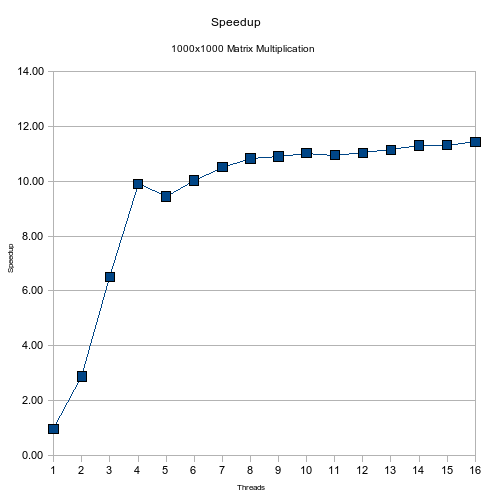
\includegraphics[width=3.3in]{shmemspeedup}
\par\end{centering}

\caption{{\footnotesize Relative speedup achieved as the number of threads
increases in our shared memory implementation. Speedup is relative
to the same Chapel code compiled with the }\emph{\footnotesize {-}{-}serial}{\footnotesize{}
flag.\label{fig:shmem_speedup}}}

\end{figure}



\subsection{Issues}

The initial goal did not involve rewriting the entire algorithm including
the BLAS implementation of GEMV but upon a survey of Chapel's interoperability
with C we concluded that it would be necessary since Chapel does not
provide enough guarantees on the representation of data. Specifically,
the standard BLAS GEMV requires array parameters to be passed as pointers
which do not exist in Chapel. This forced us to write everything including
a simplified version of the BLAS GEMV in Chapel. The immature support
for interoperability with the C language causes us to lose the benefit
of using highly optimized BLAS routines such as those found in the
widely used GotoBLAS\cite{gotoblas}.


\section{Blocked Multi-Locale GEMM Implementation\label{sec:blk-GEMM}}


\subsection{Description of Algorithm}

Even though support for multiple locales is still in its early stages
we decided to implement a blocked GEMM algorithm, $C:=AB+\hat{C}$,
that used multiple locales to evaluate the ease of reasoning about
and programming with Chapel's data locality features. The blocked
GEMM algorithm that we implemented partitions $A$ into panels along
the first dimension and the $B$ into panels along the second dimension.
The algorithm then performs a series of general panel panel multiplies,
$C:=A_{i}B_{i}+\hat{C}$. According to \cite{TSoPMC} this algorithm
performs better than the other blocked GEMM algorithms in libFLAME. 


\subsection{Implementation and Issues}

The largest roadblock that we encountered was that while the Chapel
developers intend to add support for user defined domain maps there
is currently only support for standard block distributions and standard
cyclic distributions. These were inadequate for our needs so we implemented
an algorithm that explicitly moved data between locales when necessary.
Once the appropriate data was moved to a locale we made use of the
\emph{local} construct in Chapel to explicitly tell the compiler that
all data references were local. The implementation of the \emph{local}
construct enables the compiler to perform performance optimizations
but does not statically check if the data references will be local.
In Chapel if a programmer makes a non-local reference inside a local
block a runtime error will occur. The compiler should have enough
information to be able to statically decide at compile-time if non-local
references are made and give a compile-time error instead of a runtime
error. The Chapel Language Specification 0.795 \cite{chplSpec} does
not in fact define the semantics of the \emph{local} construct but
it can be deduced from the discussion in \cite{hpcc09} that it provides
a boost in performance to explicitly assert that all references are
local.

Using the current implementation of the Chapel compiler (version 1.1)
our implementation induced much more data movement than we had intended.
When multiplying two $100\times100$ matrices with a block size of
ten our implementation induced 228,400 remote data communications.
Without the use of user defined domain maps it is very difficult to
reason about how many remote operations will be used to implement
a given statement in Chapel which results in poor performance. Figure
\ref{fig:blk_flamecomm} shows that in our implementation of the blocked
GEMM algorithm the amount of data communication grows faster than
the problem size. This would most likely not have been the case if
a user defined domain map had been used to manage our data locality.
For this reason it is too early to decide if Chapel will eventually
be able to efficiently handle the data movement involved in this blocked
GEMM algorithm.

%
\begin{figure}
\begin{centering}
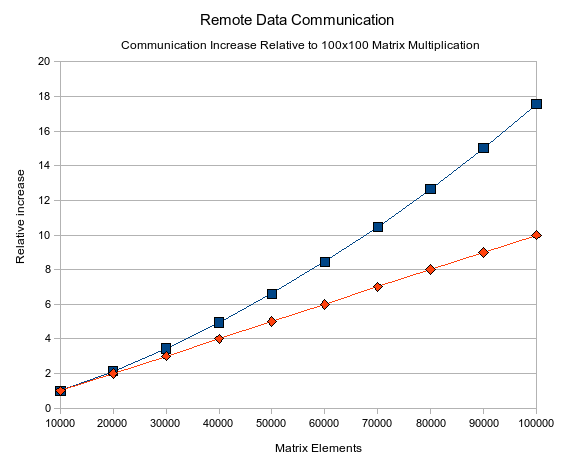
\includegraphics[width=3.3in]{blkComm}
\par\end{centering}

\caption{{\footnotesize Remote communication increases faster than the problem
size in our implementation. The red (bottom) line shows a linear increase
and the blue (top) line shows the increase observed in our implementation.\label{fig:blk_flamecomm} }}

\end{figure}



\section{SUMMA Implementation\label{sec:SUMMA-implementation}}


\subsection{Description}

Though not part of libFLAME we decided to implement a scalable matrix
multiplication algorithm called SUMMA \cite{summa}. SUMMA has a number
of benefits in that it not only achieves high performance but is also
relatively simple compared to its predecessors. This algorithm is
only practical in a parallel environment so it wouldn't make sense
for the sequential FLAME library to include it. However, the SUMMA
algorithm tests multiple facets of Chapel's programmability so its
implementation is a good exercise. The key to achieving performance
benefits with the algorithm is replication. We give a high level explanation
of the algorithm for the sake of clarity before discussing our implementation
and issues encountered. 


\subsubsection{Unblocked SUMMA}

Assume we have a group of computation nodes that can be logically
arranged into a $r\times c$ mesh, each node can be indexed by $P_{ij}$,
where $i$ is the node's row and $j$ is the node's column. To simplify
the explanation assume we have two matrices $A$ and $B$ where $A$
is $r\times n$ and $B$ is $n\times c$. In practice this simplification
can be removed by using a block-cyclic distribution along the rows
and columns of nodes. We replicate row $a_{i}$ along node row $p_{i}$
and column $b_{j}$ along node column $p_{j}$. Each node can then
perform a rank-one update in parallel to compute $C_{ij}=a_{i}*b_{j}$.
The idea is that the communication overhead for replicating each row
and column should be small compared to the performance gain achieved
by having to perform only a single rank-one update on each node. 


\subsubsection{Blocked SUMMA}

Van de Geijn and Watts \cite{summa} found that even more performance
can be achieved by formulating the computations as matrix-matrix multiplications
instead of rank-one updates. The idea is that communication is reduced
because more data is being sent to each node and smaller blocks can
take advantage of data locality better than entire rows or columns.
Our implementation of the blocked SUMMA algorithm takes in two arguments
for block size call them $s$ and $t$. It partitions matrix $A$
into $m\times t$ groups of columns, or column panels, and partitions
matrix $B$ into $t\times n$ row panels. Each panel of matrix $B$
is replicated across its respective row in the mesh of nodes. For
example, $B_{0}^{j}$, where j is the node column index, is replicated
across node row $p_{0}$. The $m\times t$ panels of matrix $A$ are
then partitioned further into $s\times t$ blocks that are block-mapped
to their corresponding logical position in the mesh of nodes. The
algorithm then performs a GEMM operation in parallel on each node
to compute block $C_{ij}=A_{ij}*B_{l}^{j}$, where $l$ is the index
of a block of rows in $B$. 


\subsection{Issues\label{sub:SUMMA-Issues}}

%
\begin{figure}
\begin{centering}
{\scriptsize
\begin{verbatim}
// replicated distributions aren't implemented yet, but imagine that
// they look something like the following:
// var replAbD: domain(2)
//                       dmapped new Dimensional(BlkCyc(blkSize),Replicated))
//                       = AbD[start.., 1..#blkSize];

// actual code to achieve the distributed replication
// Notice the replicated domains must be declared INSIDE the "on" block
for pnl in 1..n by blkcols
{
  loc1 = (loc1 + 1) % numLocales;
  loc1cnt = loc1cnt + 1;
  on Locales(loc1)
  {
    var start: int = pnl;
    var replAbD: domain(2) = AbD[1.., start..start+blkcols-1];
    var replAb : [replAD] real = Ab[1.., start..start+blkcols-1];
\end{verbatim}
 $\vdots$
}
\par\end{centering}

\centering{}\caption{{\footnotesize Example adapted from Chapel HPL HPC Challenge 2009
entry \cite{hpcc09} demonstrating how to replicate data across locales.}}
\label{Flo:ChapelReplications}
\end{figure}
We encountered significant programmability issues during all aspects
of the algorithm's implementation. Chapel's current limitations with
domain mapping forced us to do replication by placing data onto a
locale (node) explicitly using the \textquotedbl{}on\textquotedbl{}
keyword, as shown in Figure \ref{Flo:ChapelReplications}. In addition
to being difficult to read this approach meant that to compute $C$
all computation had to be done at every iteration of the innermost
loop otherwise the names of the replicated data fall out of scope
and can no longer be accessed. This also increases the communication
required to compute an answer. We would ideally like to leave $C$
partitioned over the mesh of nodes so that the only communication
cost is in the replication of data. In Chapel however, if we leave
$C$ partitioned we have no way to access $C$'s component blocks.
In order to return an answer we have to send all the computed data
from each node back to a single node that holds the original reference
to $C$. Figure \ref{fig:blk_summa} shows the increase in communication
that this incurs. Again, it would be nice to see if Chapel's user
defined domain maps could handle this algorithm elegantly, however,
at this stage in Chapel's development this was not possible.

%
\begin{figure}
\begin{centering}
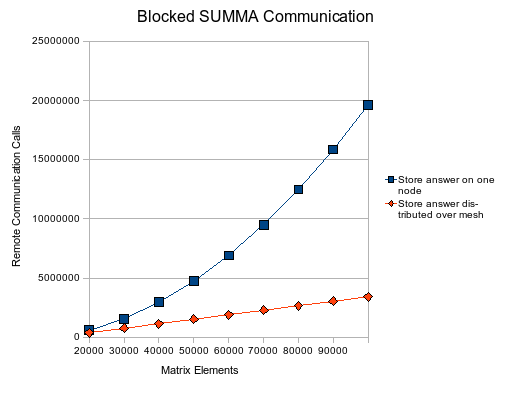
\includegraphics[width=3.8in]{blksumma_comm}
\par\end{centering}

\caption{{\footnotesize Remote communication required for our blocked SUMMA
Chapel implementation measured using the same technique as in Figure
\ref{fig:blk_flamecomm}. Squares show the large increase in communication
required to store $C$ on one node. Diamonds show communication for
the ideal case where $C$ is partitioned across the mesh of nodes.\label{fig:blk_summa}}}

\end{figure}



\section{Conclusions\label{sec:Conclusions}}

It is still too early in the development of Chapel to reach any final
conclusions regarding Chapel's ability to implement parallel linear
algebra libraries. The results from our shared memory GEMM implementation
show that relative speedup is possible as the number of threads increases
which is promising. If optimizations continue to be added to the Chapel
compiler it may become possible to achieve performance that surpasses
the sequential C implementation of libFLAME. The biggest deterrent
for library developers at this point in Chapel's development is the
lack of data locality features. The inability to create user defined
domain maps across locales is a major issue when attempting to implement
efficient linear algebra algorithms. Once this feature is implemented
in the Chapel compiler another evaluation should be conducted. In
the compiler's current state it is too difficult to manage data locality
for some of the proven parallel GEMM algorithms.

\bibliographystyle{acm} \nocite{*} \bibliographystyle{plain}
\nocite{*}
\bibliography{report}

\end{document}
